\chapter{System Model}
\label{chap:sysmodel}

\autoref{chap:background} established the standards path from application criticality through \gls{dscp} marking and IEEE~802.11 \gls{edca} to a shared contention medium, and \autoref{sec:rel_work} showed that stronger vehicular \gls{mac} alternatives typically require synchronization, infrastructure, or a different radio access technology.
The residual design point occupied by this dissertation is narrower: protect rare, high-impact crash alerts with an explicit DSCP~46-to-Voice mapping plus local, event-triggered \gls{be} suppression on IEEE~802.11p \gls{ocb} operation, without reservations, clock synchronization, or a new \gls{mac} protocol~\cite{jiang2008ieee80211p,IEEE80211,RFC8325_WiFi_QoS}.

This chapter formalizes that design point as an abstract system model---what the proposed system \emph{is}, independently of any particular simulator, programming language, or software stack.
It defines the decentralized highway network, the synthetic two-class traffic abstraction, the five \gls{mac} policies and three-mode adaptive controller, the crash-event timeline, and the modeling assumptions.
Concrete numeric bindings for timing, load, radio, and access-control knobs are recorded with the software realization in \autoref{chap:implementation}; how well the system performs under experiment is deferred to the subsequent evaluation.

The chapter is organized as follows.
Section~\ref{sec:sys:network} states the network model.
Section~\ref{sec:sys:traffic} defines the traffic classes.
Section~\ref{sec:sys:qos} presents the \gls{qos} mapping and the five \gls{mac} policies.
Section~\ref{sec:sys:event} describes the crash timeline.
Section~\ref{sec:sys:scope} lists assumptions and scope limits.

%%%%%%%%%%%%%%%%%%%%%%%%%%%%%%%%%%%%%%%%%%%%%%%%%%%%%%%%%%%%%%%%%%%%%%%%%%%%%%%%
\section{Network Model}
\label{sec:sys:network}

The system considers a decentralized vehicular ad hoc network in which vehicles communicate directly over a shared IEEE~802.11p channel.
No access point, roadside unit, or centralized coordinator participates in forwarding or channel allocation~\cite{jiang2008ieee80211p}.
All stations therefore contend for the same wireless medium under \gls{ocb} operation, so the delivery of urgent traffic depends on distributed medium access rather than on reserved transmission opportunities~\cite{IEEE80211,etsi_en_302663}.

At the application level, communication follows a one-hop multicast dissemination model: each transmission is injected into the same contention-based medium and may be received by all vehicles within radio range.
Group-addressed IEEE~802 frames inherit the hostile link-layer contract already discussed in \autoref{chap:background}---no acknowledgement, no automatic retransmission, and typically a conservative mandatory data rate---so timely delivery hinges on contention control and on correct priority mapping rather than on link-layer recovery~\cite{RFC9119_Multicast_IEEE802_Wireless}.
\autoref{fig:sys:architecture} summarizes this infrastructure-free \gls{v2v} picture.

\begin{figure}[htb]
	\caption{\label{fig:sys:architecture}System architecture: decentralized vehicle nodes communicating over IEEE~802.11p without infrastructure support.}
	\begin{center}
		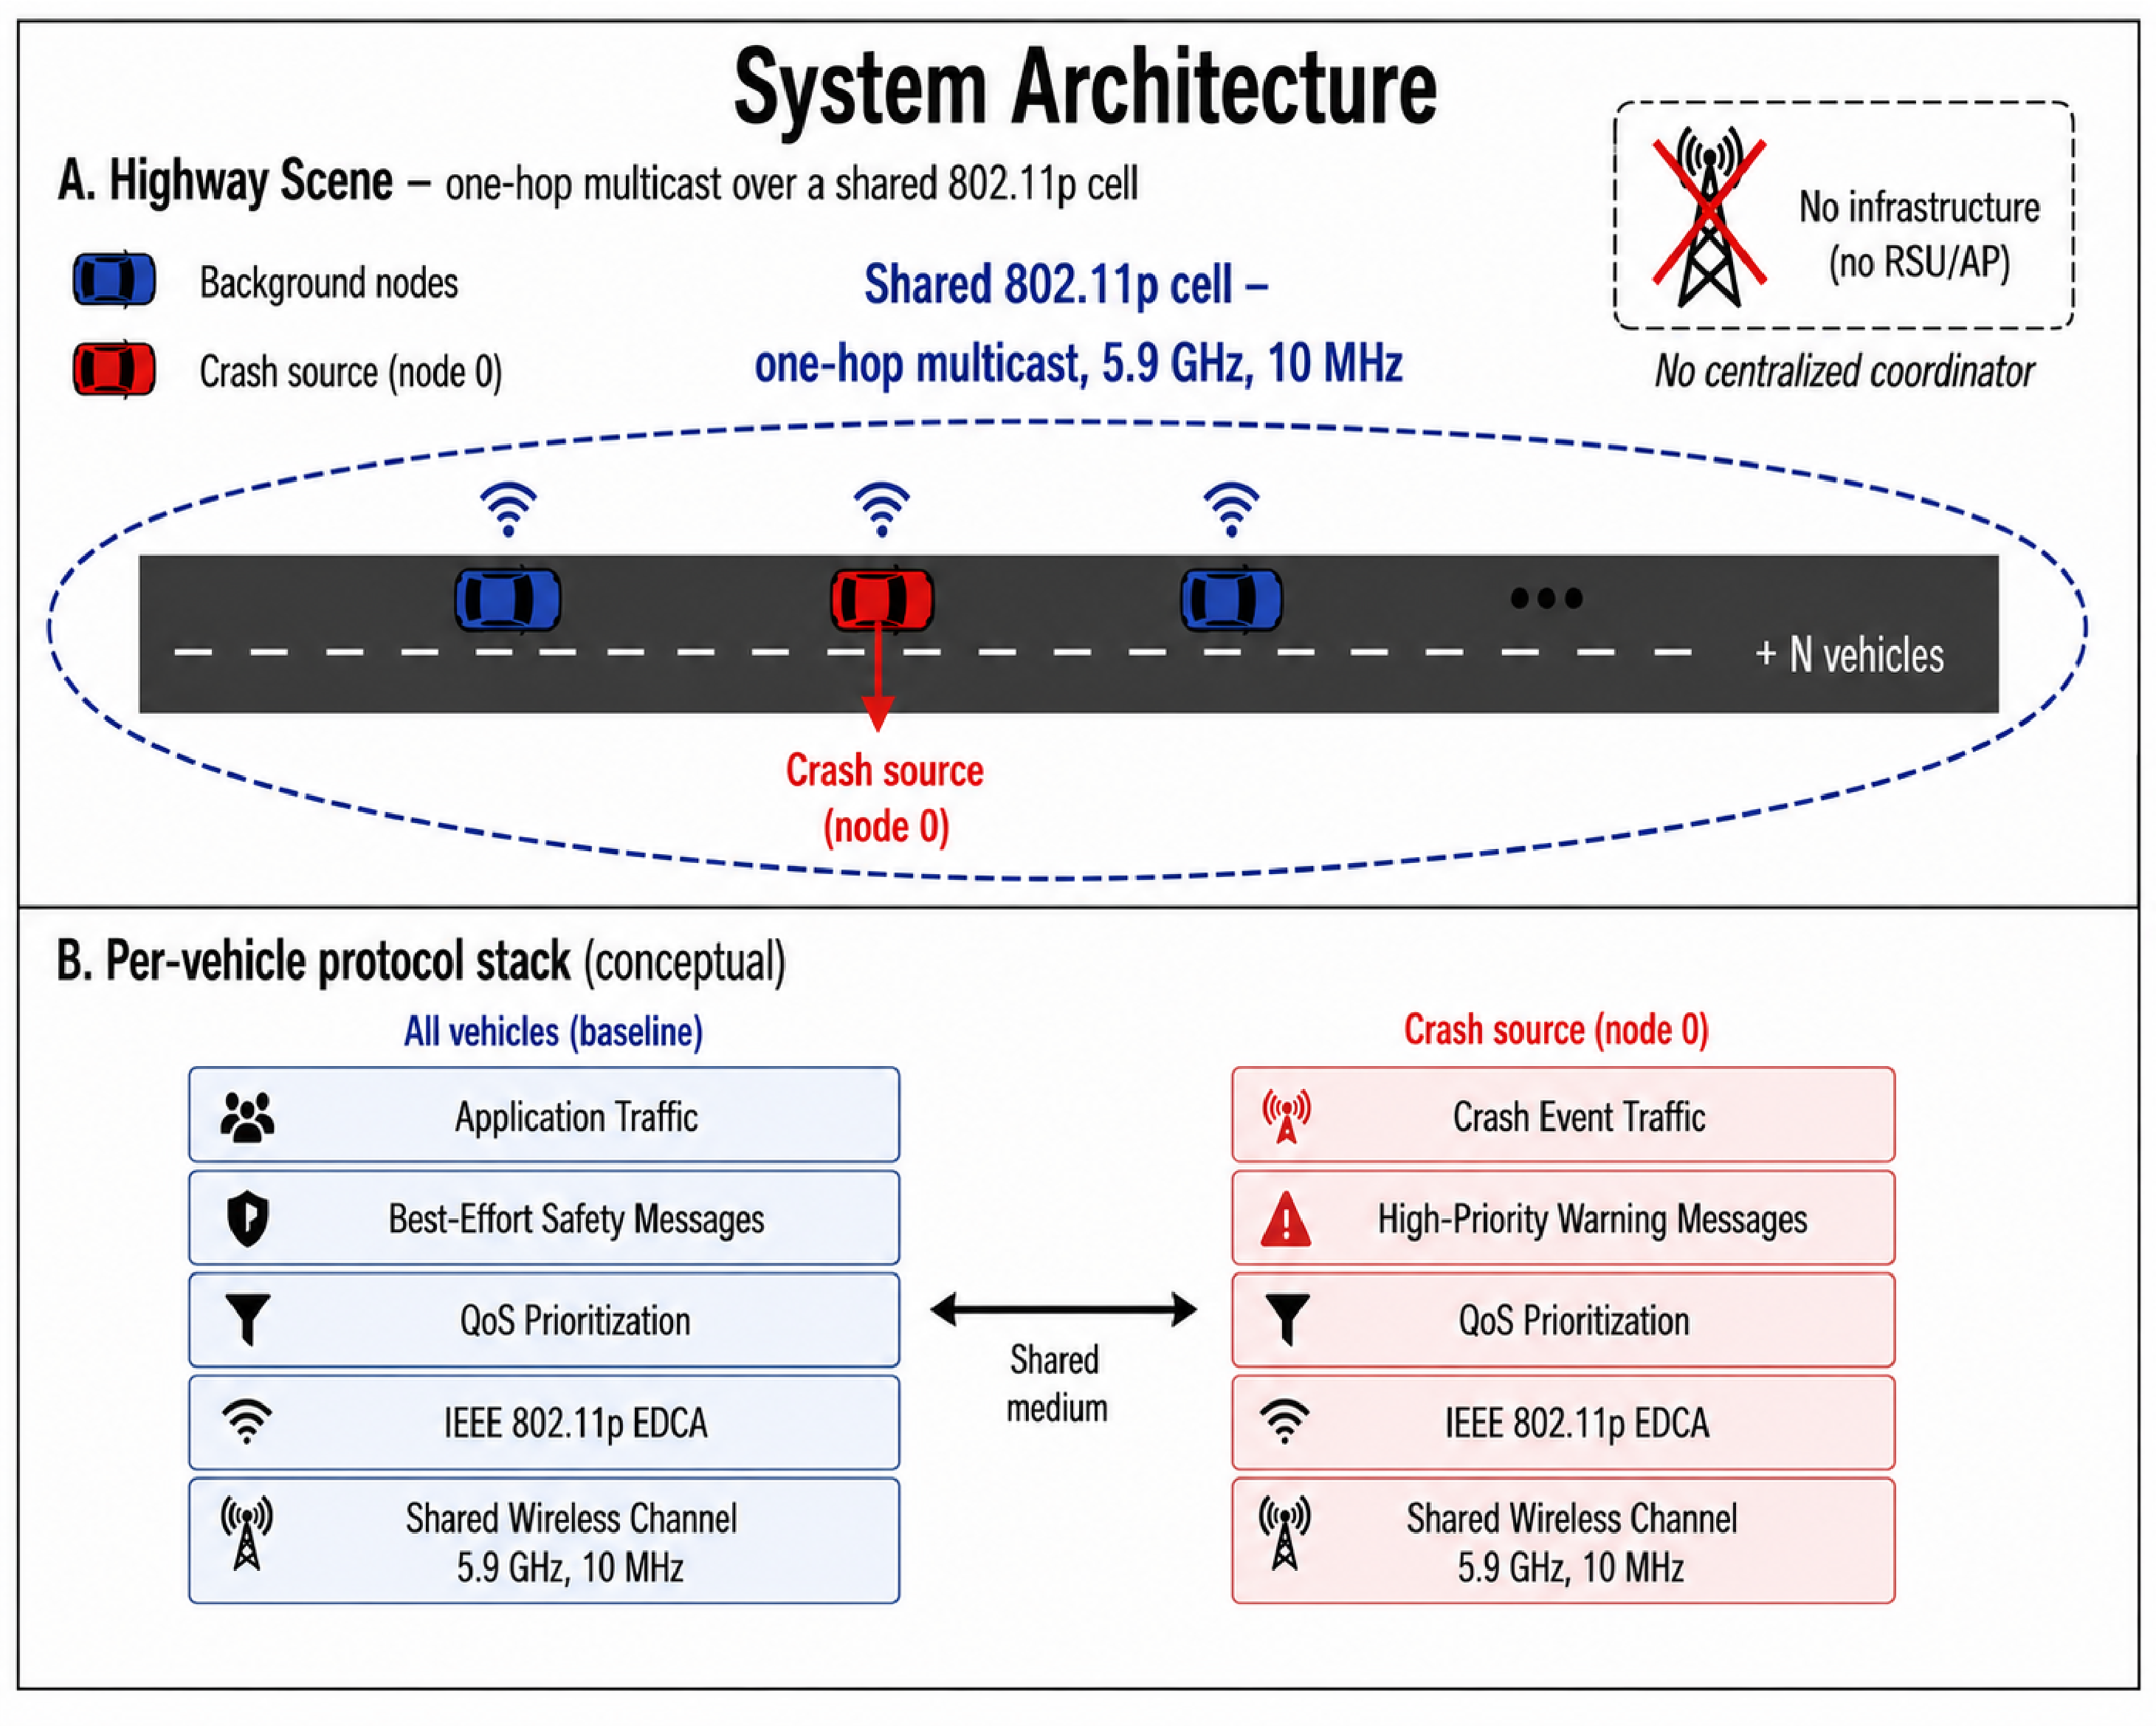
\includegraphics[width=0.92\linewidth]{Figs/system_model_architecture.pdf}
	\end{center}
	\fonte{Prepared by the author.}
\end{figure}

The radio model uses an IEEE~802.11p physical layer at 5.9~GHz with 10~MHz channelization; reference transmit power, channel index, sensitivity, noise floor, and \gls{snir} threshold are fixed for all policies and recorded with the implementation parameters in \autoref{tab:impl:parameters}.
Propagation is free-space path loss with binary obstruction and without small-scale fading or shadowing, as stated in \autoref{sec:sys:scope}.
\emph{Physical-layer connectivity is held fixed across the five \gls{mac} policies}, so differences between \gls{be} and \gls{vo} service reflect queueing and contention rather than time-varying link quality.
Dense highway broadcast already stresses this shared medium through repeated backoff freezing under load~\cite{Continuous_Backoff_Freezing_Li,bianchi2000DCF}; the model isolates that contention so that the policies can be compared under controlled offered load.

%%%%%%%%%%%%%%%%%%%%%%%%%%%%%%%%%%%%%%%%%%%%%%%%%%%%%%%%%%%%%%%%%%%%%%%%%%%%%%%%
\section{Traffic Model}
\label{sec:sys:traffic}

Traffic uses a synthetic two-class abstraction rather than standardized \gls{cam} or \gls{denm} schedules, ITS-G5 or WAVE application stacks, or production vehicular logic.
The goal is to isolate \gls{mac}-level protection-versus-cost trade-offs under controlled offered load, not to reproduce a complete \gls{its} protocol stack.

Every vehicle generates ordinary background traffic throughout the scenario horizon.
This flow represents non-critical cooperative traffic and is modeled by a configurable payload, a random inter-arrival process with a prescribed mean (exponential draws in the software artifact), and default Best Effort marking (\gls{dscp}~0).
The model instantiates this process with low, medium, and high offered-load profiles so all \gls{mac} policies face the same application-side load within a given profile; the concrete means, payloads, and Voice burst parameters appear in \autoref{tab:impl:parameters}.

Crash-alert dissemination is an event-driven overlay on that background.
One designated vehicle becomes the crash source at the configured crash time and begins emitting alert messages marked with \gls{dscp}~46, the Expedited Forwarding codepoint used in this study as the crash marker~\cite{RFC3246_EF_PHB,RFC4594_DiffServ_Service_Classes}.
Each logical alert may be repeated a configurable number of times, with configurable spacing and jitter, to represent short warning bursts.
Importantly, the crash-alert flow is \emph{superimposed} on the background flow rather than replacing it: the crash source continues to contribute ordinary \gls{be} traffic while simultaneously injecting urgent alerts.
After the crash window ends, alerts cease and the network returns to \gls{be}-only operation, as detailed in \autoref{sec:sys:event}.

%%%%%%%%%%%%%%%%%%%%%%%%%%%%%%%%%%%%%%%%%%%%%%%%%%%%%%%%%%%%%%%%%%%%%%%%%%%%%%%%
\section{QoS Model and MAC Policies}
\label{sec:sys:qos}

The model admits only two traffic classes.
Periodic background packets remain Best Effort and carry \gls{dscp}~0.
Crash-alert packets carry \gls{dscp}~46 and, in the \gls{qos}-enabled policies, are explicitly mapped to the IEEE~802.11 Voice user priority and \gls{ac}~\cite{RFC8325_WiFi_QoS,IEEE80211e_2005}.
That mapping is not automatic in every stack; the Background chapter's DiffServ path (\autoref{sec:bg:dscp}) is the normative mapping assumed here for QoS-enabled policies~\cite{RFC2474_DSField,RFC2475_DiffServ_Architecture}.
\autoref{fig:sys:stack} summarizes the abstract end-to-end path from application marking to channel access.

\begin{figure}[htb]
	\caption{\label{fig:sys:stack}Conceptual cross-layer path for crash-aware prioritization. Study-specific mechanisms act at Application, Network/\gls{qos}, and \gls{mac}; the shared \gls{phy} baseline is identical across all policies.}
	\begin{center}
		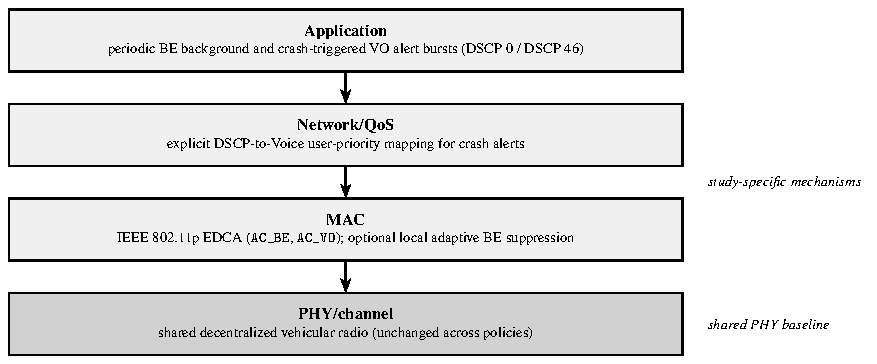
\includegraphics[width=0.95\linewidth]{Figs/sys_stack.pdf}
	\end{center}
	\fonte{Prepared by the author.}
\end{figure}

Five \gls{mac} policies operate on the same traffic and radio model.
They form a comparison ladder from undifferentiated access, through standard \gls{edca} differentiation, to three adaptive extensions that temporarily suppress competing \gls{be} traffic while crash alerts are active.
None of the policies reserves the channel or claims deterministic delay bounds: \gls{edca} provides statistical differentiation only~\cite{mangold2003QoS,kosekszott2012What,kong2004EDCA}.

\begin{itemize}
  \item \texttt{plain} --- Non-\gls{qos} \gls{dcf} baseline: undifferentiated access with a single pending queue and no DSCP-to-\gls{ac} mapping~\cite{IEEE80211,bianchi2000DCF}.
  \item \texttt{edca\_only} --- Standard \gls{qos} baseline: \gls{dscp}~46 maps to \texttt{AC\_VO}; all other packets use user priority~0~\cite{IEEE80211e_2005}.
  \item \texttt{edca\_v2x\_vo\_stable} --- Sustained Voice protection: inherits \texttt{edca\_only} and adds the adaptive controller below with comparatively long protection windows.
  \item \texttt{edca\_v2x\_vo\_guarded} --- Bounded suppression: same inheritance with tighter, shorter protection windows.
  \item \texttt{edca\_v2x\_vo\_emergency} --- Emergency preemption: same inheritance with aggressive activation; newly arriving \gls{be} packets may be dropped while protection is active.
\end{itemize}

\noindent
For brevity the adaptive policies are often abbreviated \texttt{stable}, \texttt{guarded}, and \texttt{emergency}.
Queue depths, contention windows, and controller timing knobs for each policy are bound in the implementation and listed in \autoref{tab:impl:parameters}.

\subsection{Adaptive three-mode controller}
\label{sec:sys:controller}

The three adaptive policies add a local three-mode \gls{fsm}---\emph{listening}, \emph{blocking}, and \emph{sending}---that temporarily gates \gls{be} eligibility for channel access without changing the underlying queue parameters inherited from \texttt{edca\_only}.
\autoref{fig:sys:fsm} summarizes the modes and transitions.

\begin{figure}[htb]
	\caption{\label{fig:sys:fsm}Local adaptive controller modes and transitions for the \texttt{edca\_v2x\_vo\_*} policies.}
	\begin{center}
		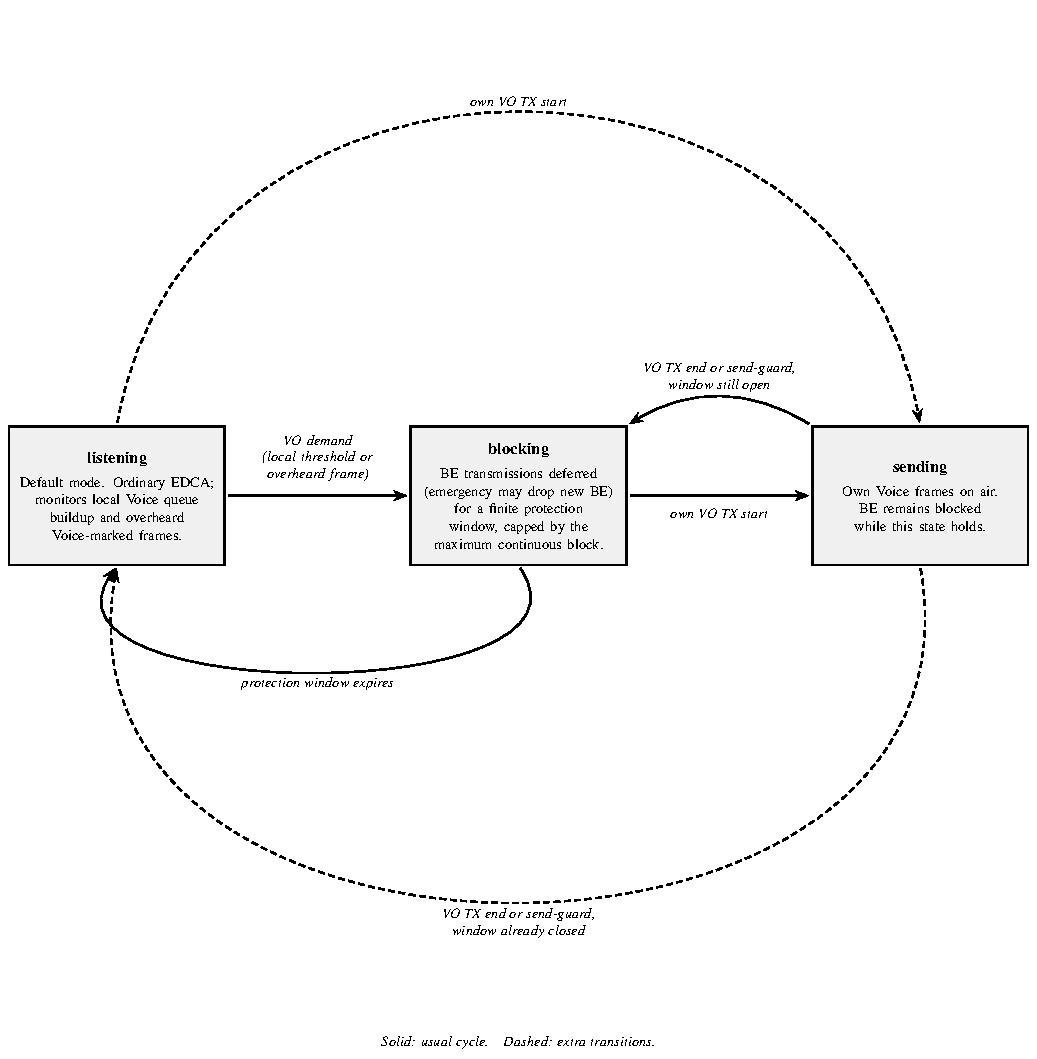
\includegraphics[width=0.95\linewidth]{Figs/sys_fsm.pdf}
	\end{center}
	\fonte{Prepared by the author.}
\end{figure}

A node leaves \emph{listening} for \emph{blocking} when the local Voice queue crosses the activation threshold or when any Voice-marked frame is overheard---a single overheard alert frame suffices to arm or extend protection; the queue threshold applies only to locally generated Voice traffic.
It moves to \emph{sending} when its own Voice frames obtain the channel.
After the Voice transmission ends---or if the send-guard timer fires first---it returns to \emph{blocking} while the protection window is still open, and to \emph{listening} once that window has expired.
Nodes that only overhear Voice traffic never enter \emph{sending}: they remain in \emph{blocking} until the window expires.
\autoref{fig:sys:fsm} also shows a skip from \emph{listening} directly to \emph{sending} when a local Voice frame wins the channel without a prior demand-triggered block.
Under \texttt{stable} and \texttt{guarded}, \gls{be} packets remain queued but lose channel-access eligibility while the controller is blocking or sending.
Under \texttt{emergency}, newly arriving \gls{be} packets may additionally be dropped and stale \gls{be} transmission opportunities released.
The mechanism shapes local contention during the alert period; it does \emph{not} reserve the medium, open scheduled gates, or provide worst-case latency bounds~\cite{IEEE80211e_2005,kosekszott2012What}.

%%%%%%%%%%%%%%%%%%%%%%%%%%%%%%%%%%%%%%%%%%%%%%%%%%%%%%%%%%%%%%%%%%%%%%%%%%%%%%%%
\section{Event Model}
\label{sec:sys:event}

The system evolves through three phases, illustrated in \autoref{fig:sys:timeline}.

\begin{figure}[htb]
	\caption{\label{fig:sys:timeline}Conceptual event timeline: normal background traffic, crash-triggered Voice prioritization, and recovery.}
	\begin{center}
		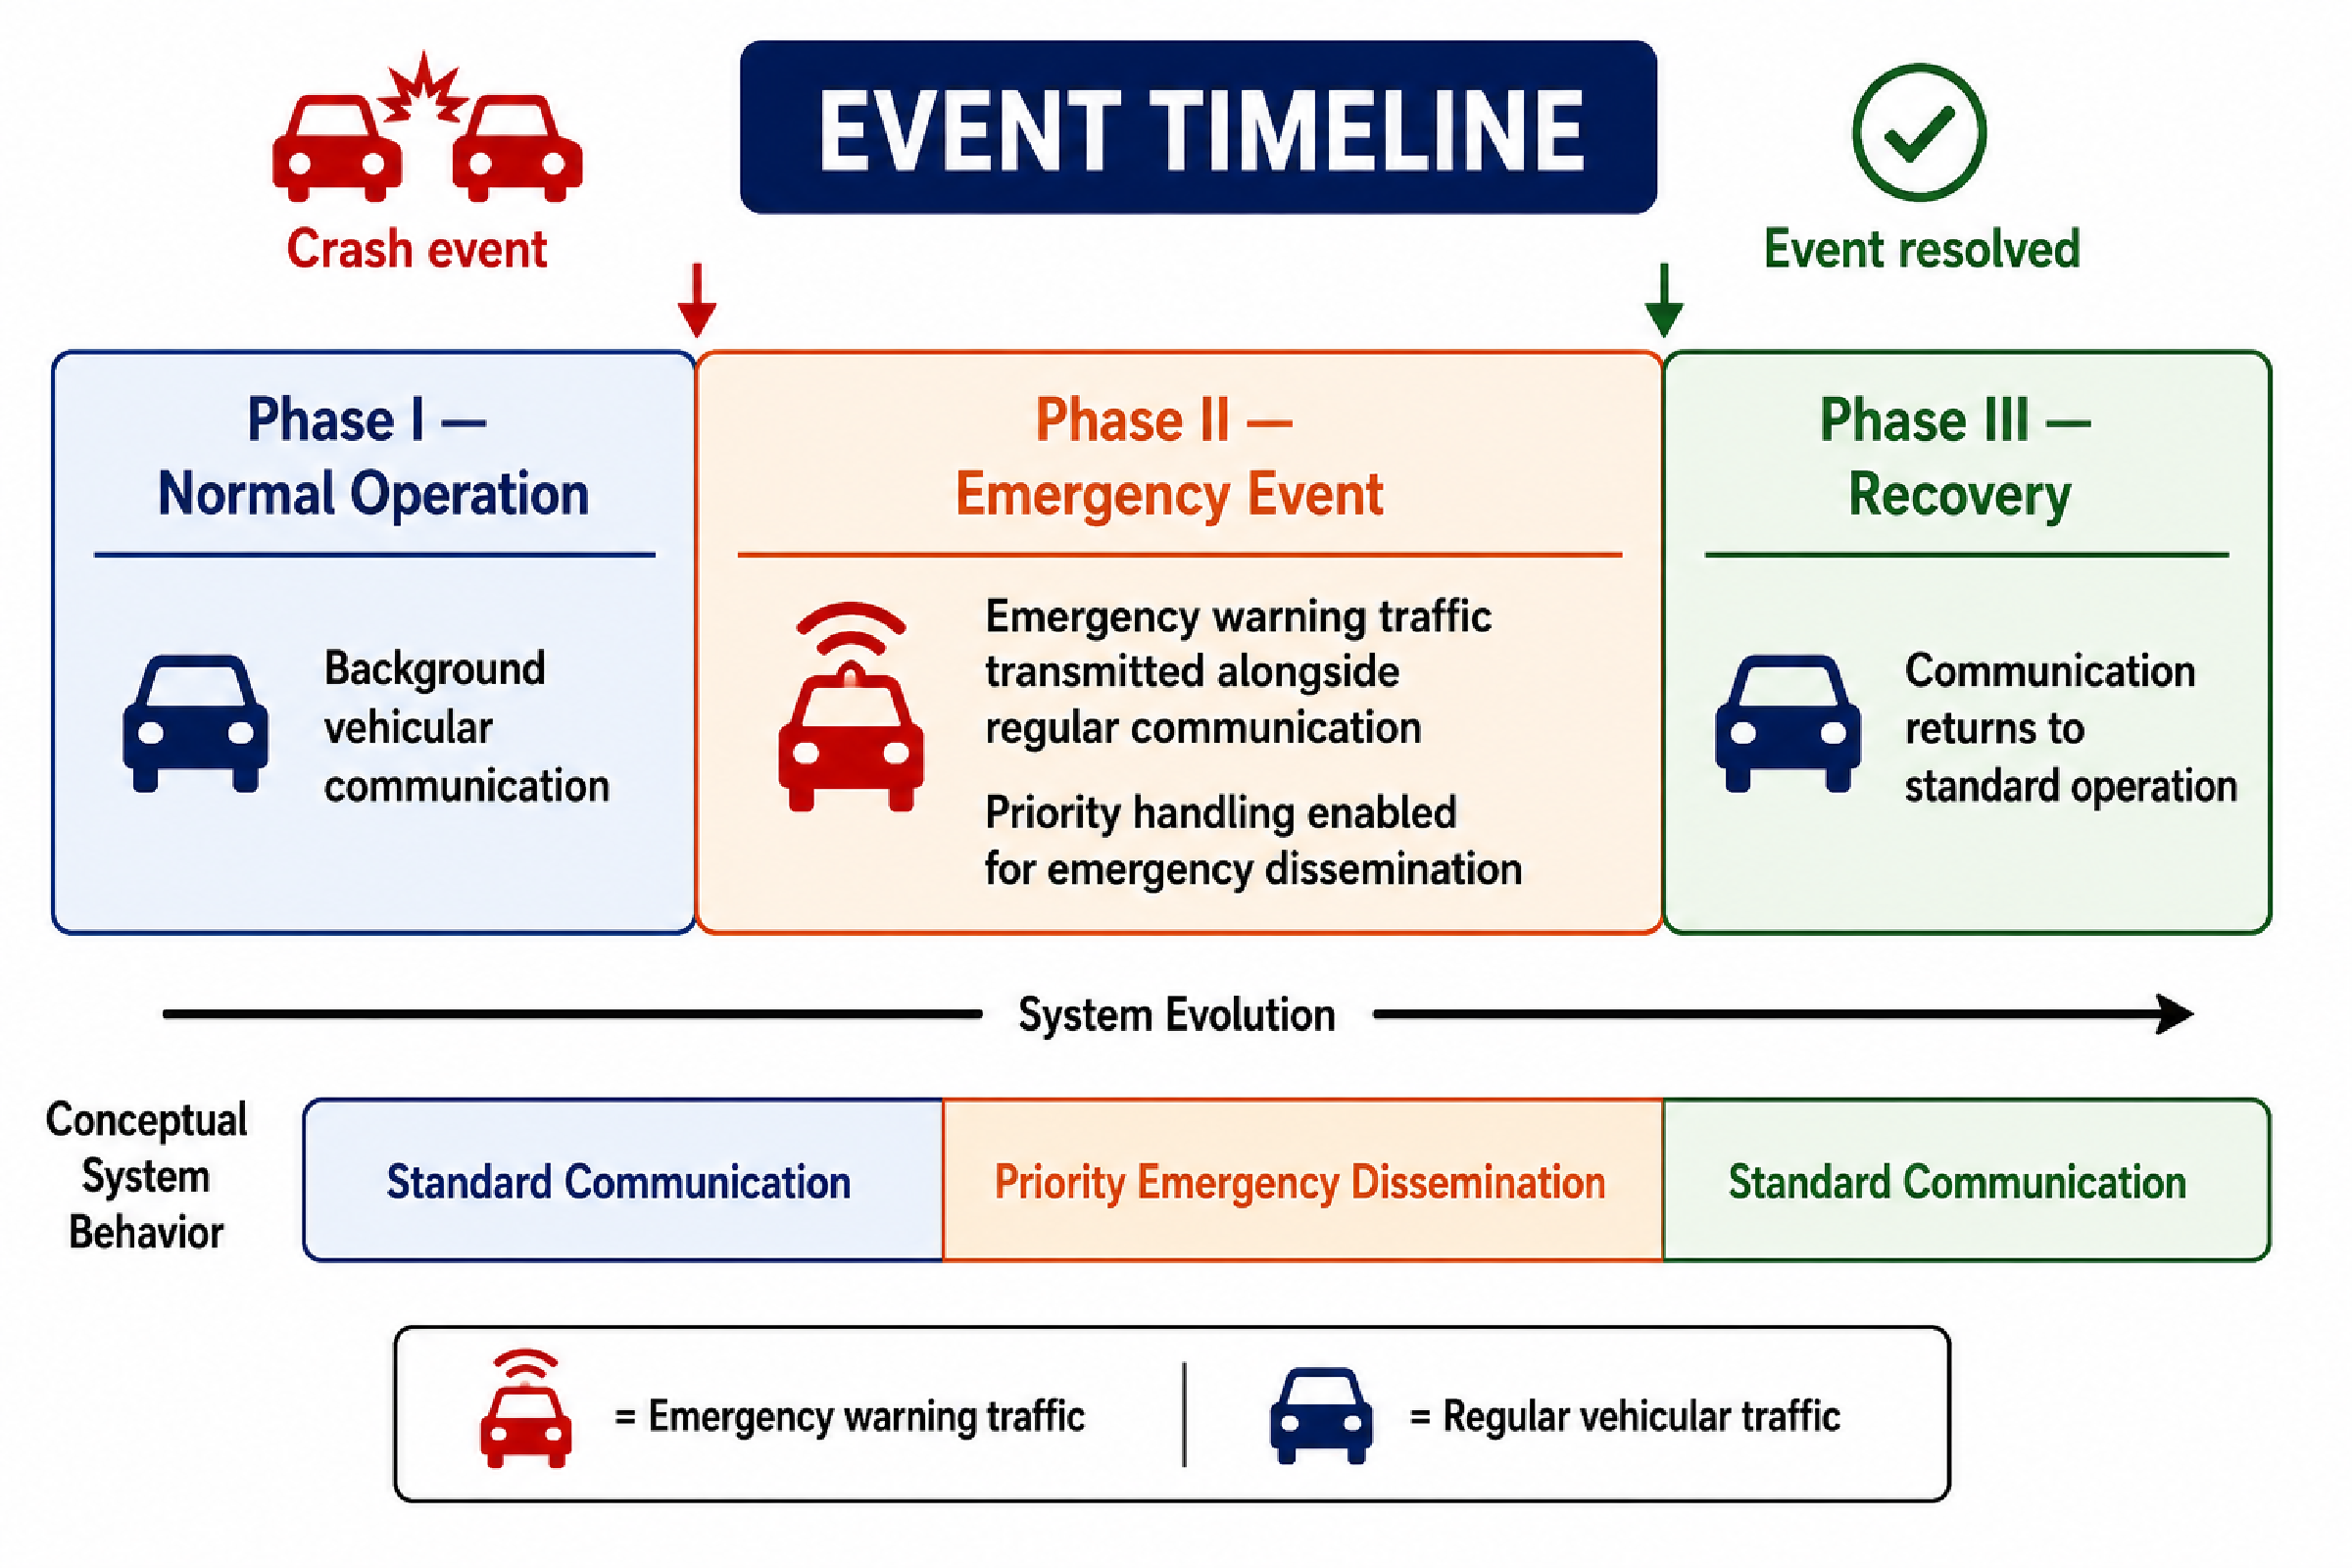
\includegraphics[width=\linewidth]{Figs/event_timeline_cropped.pdf}
	\end{center}
	\fonte{Prepared by the author.}
\end{figure}

\begin{enumerate}
  \item \textbf{Normal operation.}
    Before the crash event, all vehicles generate only periodic \gls{be} multicast traffic.
    No crash-alert Voice flow is present, and adaptive controllers remain in \emph{listening}.
  \item \textbf{Crash window.}
    At time~\SI{30}{\second} of the scenario horizon, one designated vehicle enters the crash state: it becomes stationary and immediately begins the Voice alert flow for a~\SI{30}{\second} window.
    Ordinary background traffic remains active across the network, including at the crash source, so urgent packets must compete with existing channel load~\cite{RFC9119_Multicast_IEEE802_Wireless}.
  \item \textbf{Recovery.}
    After the crash window expires, crash-alert transmissions cease and the system reverts to \gls{be}-only background traffic.
    Under the adaptive policies, however, the local effect of the crash can briefly outlast the application burst: nodes that still observe Voice queue pressure or receive crash-related Voice frames may remain temporarily in \emph{blocking} or \emph{sending} until the protection window and its short guard interval expire.
\end{enumerate}

This three-phase structure is deliberately simple.
It isolates a single crash source and a bounded alert interval so that the five policies can be compared on the same timeline under light and heavy fleet densities.

%%%%%%%%%%%%%%%%%%%%%%%%%%%%%%%%%%%%%%%%%%%%%%%%%%%%%%%%%%%%%%%%%%%%%%%%%%%%%%%%
\section{Assumptions and Scope}
\label{sec:sys:scope}

The model is intentionally minimal.
There is no infrastructure, centralized scheduler, or Time-Sensitive Networking-style gating; there is a single crash source; and there is a two-class \gls{be}/\gls{vo} distinction only.
Road geometry, fleet density, and radio parameters fix concrete instances of the model; their reference values are recorded with the implementation in \autoref{tab:impl:parameters}.

\gls{dcc}, as standardized for ITS-G5 deployments, is \emph{not} part of the model: application transmit rates follow the fixed offered-load profiles rather than reacting to channel busy ratio~\cite{etsi_dcc_2018}.
As argued in \autoref{sec:rel_work}, DCC remains a complementary always-on regulator; excluding it here isolates the protection-versus-cost behaviour of the five \gls{mac} policies.

Small-scale fading, log-normal shadowing, and graded obstacle attenuation are likewise omitted.
Connectivity uses free-space path loss, a static \gls{snir} threshold, and binary obstruction (a link is either clear or fully blocked).
Contention is therefore induced mainly by multicast load and fleet density, so the policies compete on backoff, queue service, and local \gls{be} suppression rather than on cross-layer load regulation or time-varying \gls{phy} stress.

Finally, the model makes no deterministic or worst-case latency claims.
\gls{edca} and all five policies provide statistical service only~\cite{kosekszott2012What,mangold2003QoS}.
Any quantitative statements about Voice or Best Effort delay belong to the evaluation, not to closed-form bounds derived from this chapter.

Together, the network, traffic, \gls{qos}, event, and scope definitions constitute the crash-aware system studied in the remainder of this dissertation.
\autoref{chap:implementation} maps the model onto a concrete software realization and records the numeric parameter bindings used in the artifact; the evaluation then asks whether crash-triggered Voice traffic obtains better wireless service than ordinary Best Effort under contention, and what cost that protection imposes on ordinary traffic.
